\documentclass{beamer}
\usetheme[titleformat=allsmallcaps]{metropolis}
\usepackage{braket}
\usepackage{graphicx}
\usepackage{tikz}
\usetikzlibrary{calc}
\usetikzlibrary{arrows,chains,matrix,positioning,scopes}
\tikzstyle{startstop} = [rectangle, minimum width=3cm, minimum height=.6cm,text centered, draw=black]
\tikzstyle{io} = [rectangle,minimum width=3cm, minimum height=.6cm, text centered, fill=hotdog]
\tikzstyle{line}=[draw, very thick, color=black!75, -latex']

\setbeamerfont{footnote}{size=\tiny}


\newrobustcmd*{\footfullcitenm}{%
  \AtNextCite{%
    \let\thefootnote\relax
    \let\mkbibfootnote\mkbibfootnotetext}%
  \footfullcite}

\definecolor{hotdog}{HTML}{e5bc14}

\title{Hartree-Fock}
% \subtitle{Group meeting presentation}
\author{Amanda Dumi}
\date{\today}

\begin{document}
\begin{frame}
\titlepage
\end{frame}

\section{background}


\begin{frame}{slater determinant}
  We need a wavefunction consisting of:
  \begin{itemize}
      \item orthogonal wavefunctions of individual particles
      \item follow antisymmetry requirement
  \end{itemize}
  $$\Phi = \frac{1}{\sqrt{N!}}
  \begin{vmatrix}
  \chi_1(x_1) & \chi_2(x_1) & \cdots & \chi_N(x_1) \\
  \chi_1(x_2) & \chi_2(x_2) & \cdots & \chi_N(x_2) \\
  \vdots & \vdots & \ddots & \vdots \\
  \chi_1(x_N)& \chi_2(x_N) & \cdots & \chi_N(x_N)
  \end{vmatrix}
  $$
\end{frame}



\begin{frame}{Realm of methods}
Exact answer:
  $$\Psi\ =\ \sum\limits_K^\infty D_k \Phi_K$$
 Hartree-Fock instead uses a single slater determinant for the ground state
    $$ \Psi = \Phi_0$$
All effort goes towards finding the best set of orbitals.

\end{frame}

\begin{frame}{self consistent field}
% \tikzstyle{every picture}+=[remember picture]

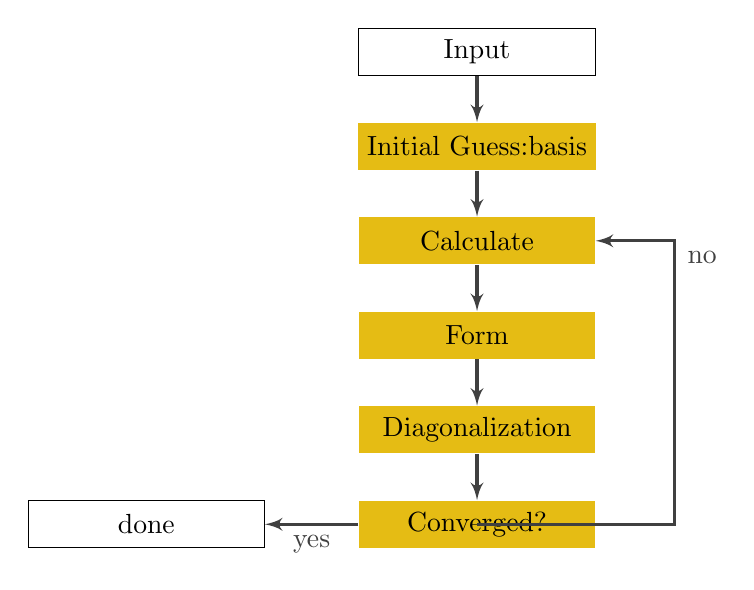
\begin{tikzpicture}[node distance=1.2cm,auto]
  \node (start) [startstop] {Input};
  \node (init) [io, below of=start] {Initial Guess:\\basis};
  \draw [line] (start) -- (init);
  \node (calc) [io, below of=init] {Calculate};
  \draw [line] (init) -- (calc);
  \node (form) [io, below of=calc] {Form};
  \draw [line] (calc) -- (form);
  \node (diag) [io, below of=form] {Diagonalization};
  \draw [line] (form) -- (diag);
  \node (conv) [io, below of=diag] {Converged?};
  \draw [line] (diag) -- (conv);
  \path [line] (conv) |- ($(conv.east) +  (1,0)$) |- node [xshift = 10pt] {no} (calc);
  \node (done) [startstop, left of=conv,node distance=4.2cm] {done};
  \path [line] (conv) -- node {yes} (done);

\end{tikzpicture}
\end{frame}


\section{algorithm}


\begin{frame}{derivation}

\end{frame}

\section{example}
\begin{frame}{background}

\end{frame}

\section{Can we improve?}
\begin{frame}{missing correlation energy}

\end{frame}
\begin{frame}{correlation energy}

\end{frame}


\end{document}
